\subsection{Análisis de cluster}
\begin{frame}{Métodos no supervisados}
\begin{columns}
\begin{column}{0.9\textwidth}
\textbf{Objetivo:} Agrupar en grupos homogéneos o \emph{clusters} las observaciones o mediciones.

\begin{defi}
Diremos que un \emph{cluster} o conglomerado es un subconjunto de las observaciones que son similares entre sí. 
\end{defi}

Se dice que dos observaciones $\mathbf{x}_i,\mathbf{x}_{i'}$ están relacionadas, $\mathcal{R}$, cuando pertenecen al mismo \emph{cluster}.

\begin{defi}
Se llama \textit{clustering} a la partición que provoca la relación $\mathcal{R}$ del espacio de observaciones. 
\end{defi}

\end{column}
\end{columns}
\end{frame}

\begin{frame}{Métodos no supervisados}
\begin{columns}
\begin{column}{0.9\textwidth}
Tipos de algoritmos de \emph{clustering}:
\begin{itemize}
\item \textbf{Particional} una única partición que se va modificando
\item \textbf{Jerárquico} otorga las posibles particiones desde $N$ \emph{cluster} hasta un sólo \emph{cluster}.
\begin{itemize}
\item \textbf{Aglomerativo: } se empiezan con $N$ \emph{clusters} con una observación en cada uno y se van juntando según un criterio establecido. 
\item \textbf{Divisivo} se empiezan con un \emph{cluster} con todas las observaciones  y se va dividiendo según algún criterio establecido. 
\end{itemize}
\end{itemize}
\end{column}
\end{columns}
\end{frame}

\begin{frame}{Métodos no supervisados}
\begin{columns}
\begin{column}{0.9\textwidth}

Dependiendo de cómo se definan las distancias entre los \emph{clusters} se obtendrá un algoritmo u otro:\\
\begin{itemize}
\item El vecino más proximo: $d(C,C')=\min_{\mathbf{x}_i\in C, \mathbf{x}_{i'}\in C'}(\mathbf{x}_i,\mathbf{x}_{i'})$.
\item El vecino más lejano: $d(C,C')=\max_{\mathbf{x}_i\in C, \mathbf{x}_{i'}\in C'}(\mathbf{x}_i,\mathbf{x}_{i'})$.
\item Enlace medio \begin{equation}
d(C,C')=\dfrac{1}{N_C}\dfrac{1}{N_C'}\sum_{\mathbf{x}_i\in C}\sum_{\mathbf{x}_{i'}\in C'} d(\mathbf{x}_i, \mathbf{x}_{i'}).
\end{equation}

\item Ward:
\begin{equation}
d(C,C')=\dfrac{1}{N_C}\dfrac{1}{N_C'}\sum_{\mathbf{x}_i\in C}\sum_{\mathbf{x}_{i'}\in C'} (d(\mathbf{x}_i, \mathbf{x}_{i'}))^2
\end{equation} 
\end{itemize}

\end{column}
\end{columns}
\end{frame}

\begin{frame}{Métodos no supervisados}
\begin{columns}
\begin{column}{0.9\textwidth}

El proceso que siguen los algoritmos jerárquicos aglomerativos es el siguiente:

\begin{itemize}
\item Se inicia con una partición que tiene $N$ \emph{clusters} con una única observación cada uno.
\item Se calcula la matriz de distancias entre los \emph{clusters}. 
\item Se unen los dos clusters que menor distancia tengan entre ellos. De esta manera, se reduce el número de clusters en 1.  
\item Se repiten los dos pasos anteriores hasta tener un único cluster. 
\end{itemize}
\end{column}
\end{columns}
\end{frame}

\begin{frame}{Métodos no supervisados}
\begin{columns}
\begin{column}{0.9\textwidth}
Estos algoritmos tienen la característica que permiten representar sus resultados como un dendograma.

\begin{defi}
Un dendograma es un diagrama de árbol en el que en el eje horizontal se sitúan las observaciones mientras que en el eje vertical se representan las distancias. Cada nodo representa una unión de los clusters. 
\end{defi}

\end{column}
\end{columns}
\end{frame}

\begin{frame}{Métodos no supervisados}
\begin{columns}
\begin{column}{0.9\textwidth}

Los siguientes dendogramas \ref{fig:complete_linkage} \ref{fig:single_linkage}  son resultado de aplicar un algoritmo jerárquico al conjunto \emph{IRIS} de Fisher.
\begin{figure}[h]
 \centering
  \subfloat[Enlace completo]{
   \label{fig:complete_linkage}
    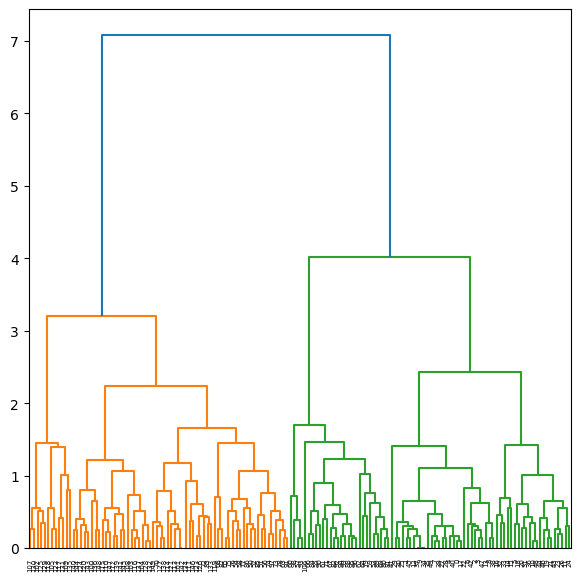
\includegraphics[width=0.35\textwidth]{Documentos Extra/Imagenes/complete_linkage.png}}
  \subfloat[Enlace simple]{
   \label{fig:single_linkage}
    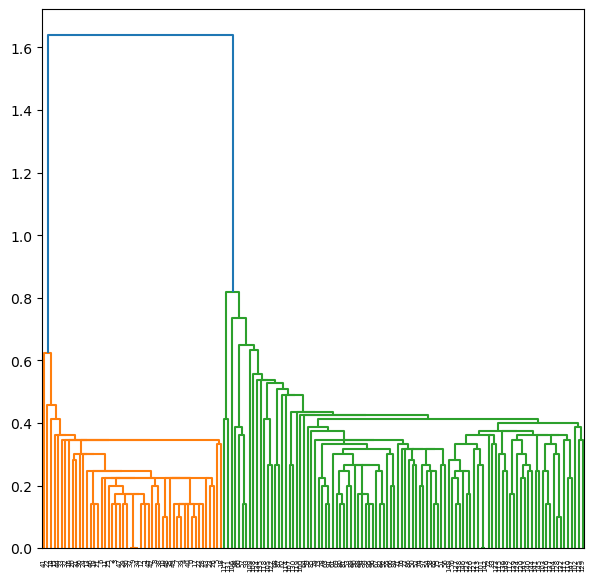
\includegraphics[width=0.35\textwidth]{Documentos Extra/Imagenes/single_linkage.png}}
 \caption{Diagramas obtenidos utilizando la biblioteca de Python Scikit-Learn}
 \label{fig:Dendogramas distintos enlaces }
\end{figure}
\end{column}
\end{columns}
\end{frame}
\begin{frame}{Métodos no supervisados}
\begin{columns}
\begin{column}{0.9\textwidth}

Como se ha dicho, los algoritmos particionales generan un único \emph{clustering} que se va modificando a lo largo de la ejecución del algoritmo.  

Para poder dar el algoritmo más importante de este tipo se necesita del siguiente concepto:

\begin{defi}
Se llama \emph{centroide} de un cluster $C_k,\enspace k=1,\ldots,K$ al vector de tamaño $p$ cuyas componentes son las medias de cada una de las variables de todas las observaciones del \emph{cluster} $C_k$:
\begin{equation}
\overline{x}_{jk}=\dfrac{1}{|C_k|}\sum_{i\in C_k}  x_{ij} \quad \forall j=1,\ldots, p
\end{equation}
\end{defi}
\end{column}
\end{columns}
\end{frame}

\begin{frame}{Métodos no supervisados}
\begin{columns}
\begin{column}{0.9\textwidth}

El algoritmo de $K$-medias se desarrolla de la siguiente manera:

 \begin{enumerate}
\item Se asignan a cada una de las observaciones en cada uno de los $K$ \emph{clusters}. Se calculan los centroides de dichos \emph{clusters}.
\item Se comprueba la distancia euclídea de cada una de las observaciones a los centroides de los \emph{clusters} y se reasignan las observaciones de acuerdo al  más cercano. Tras esto se recalculan los centroides.
\item Se repiten los dos pasos anteriores hasta que las asignaciones no cambien. 
\end{enumerate}
\end{column}
\end{columns}
\end{frame}

